\section{FDPStar  Class Reference}
\label{class_FDPStar}\index{FDPStar@{FDPStar}}
An A-Star search variant. The Metric in {\bf Problem} {\rm (p.\,\pageref{class_Problem})} is used as the cost. 


{\tt \#include $<$fdp.h$>$}

Inheritance diagram for FDPStar::\begin{figure}[H]
\begin{center}
\leavevmode
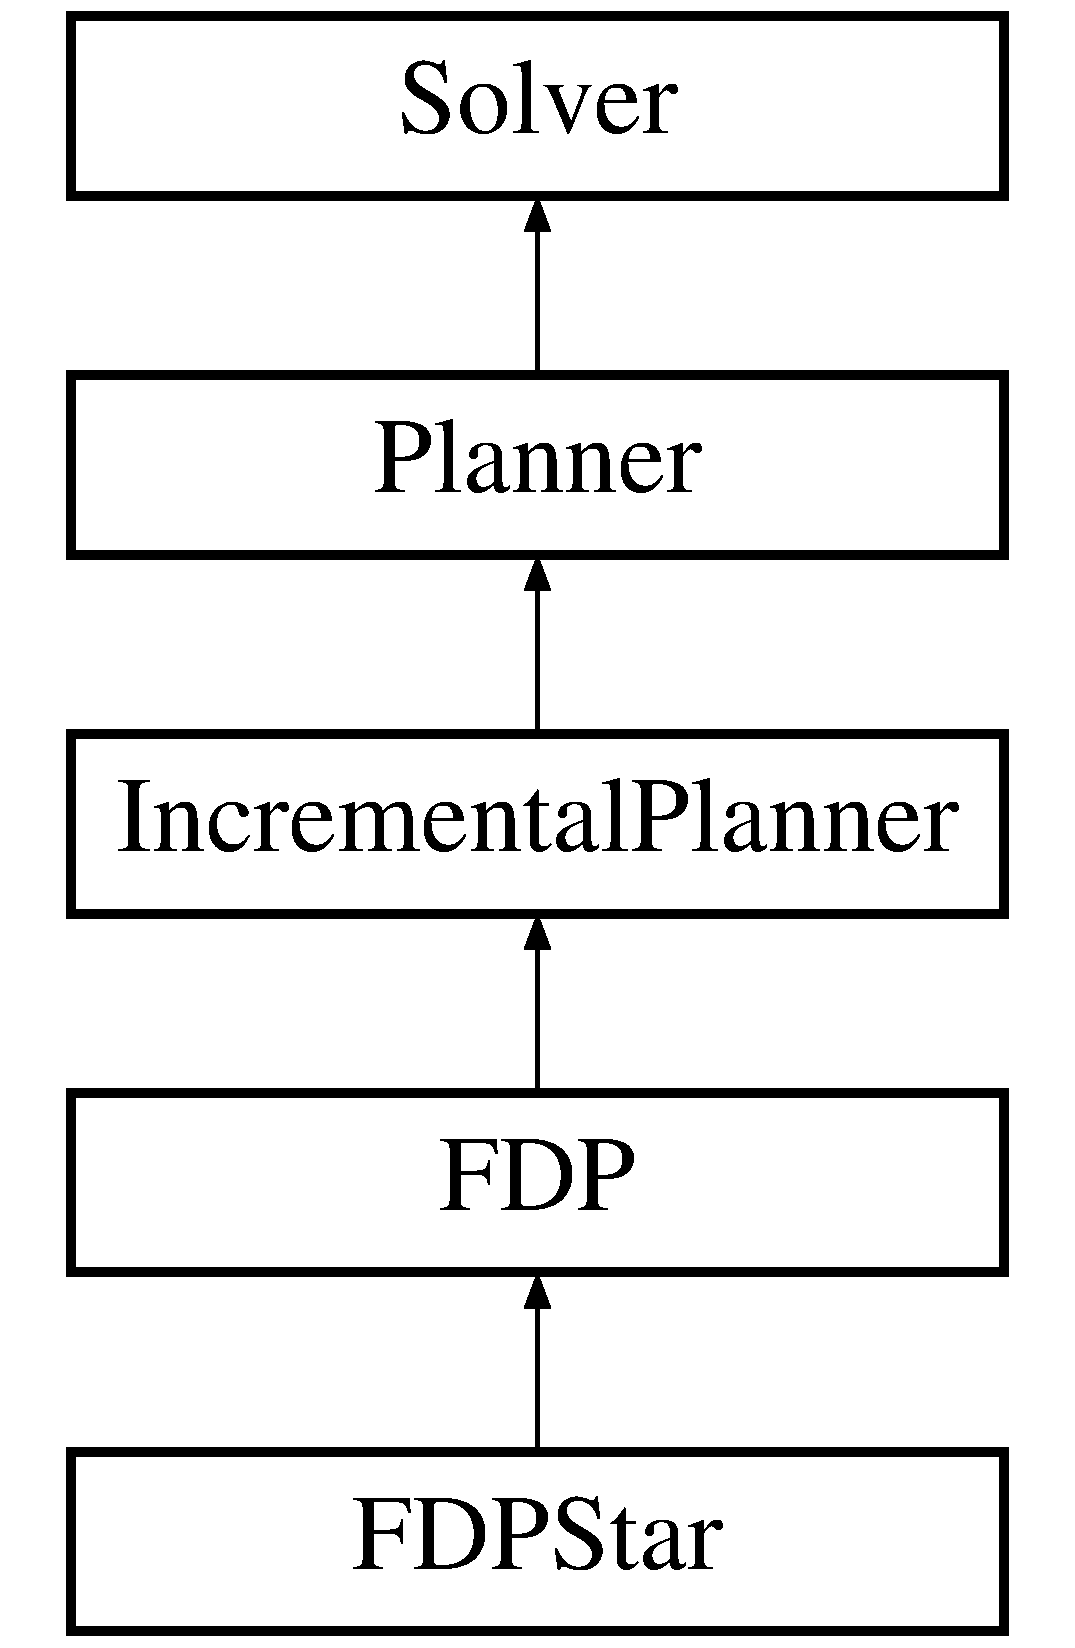
\includegraphics[height=5cm]{class_FDPStar}
\end{center}
\end{figure}
\subsection*{Public Methods}
\begin{CompactItemize}
\item 
{\bf FDPStar} ({\bf Problem} $\ast$p)
\end{CompactItemize}
\subsection*{Protected Methods}
\begin{CompactItemize}
\item 
virtual double {\bf Search\-Cost} (double initcost, {\bf MSLNode} $\ast$\&n, {\bf MSLNode} $\ast$\&nn)
\end{CompactItemize}


\subsection{Detailed Description}
An A-Star search variant. The Metric in {\bf Problem} {\rm (p.\,\pageref{class_Problem})} is used as the cost.



\subsection{Constructor \& Destructor Documentation}
\index{FDPStar@{FDPStar}!FDPStar@{FDPStar}}
\index{FDPStar@{FDPStar}!FDPStar@{FDPStar}}
\subsubsection{\setlength{\rightskip}{0pt plus 5cm}FDPStar::FDPStar ({\bf Problem} $\ast$ {\em p})}\label{class_FDPStar_a0}




\subsection{Member Function Documentation}
\index{FDPStar@{FDPStar}!SearchCost@{SearchCost}}
\index{SearchCost@{SearchCost}!FDPStar@{FDPStar}}
\subsubsection{\setlength{\rightskip}{0pt plus 5cm}virtual double FDPStar::Search\-Cost (double {\em initcost}, {\bf MSLNode} $\ast$\& {\em n}, {\bf MSLNode} $\ast$\& {\em nn})\hspace{0.3cm}{\tt  [protected, virtual]}}\label{class_FDPStar_b0}




Reimplemented from {\bf FDP} {\rm (p.\,\pageref{class_FDP_b0})}.

The documentation for this class was generated from the following file:\begin{CompactItemize}
\item 
{\bf fdp.h}\end{CompactItemize}
